\documentclass{beamer}
\usepackage[utf8]{inputenc}
\usepackage[spanish]{babel}
\usepackage{hyperref}
\usepackage{verbatim}
\usepackage{listings}
\usepackage{tikz}
\usepackage{ulem}
\usepackage{graphicx}
\usepackage{booktabs}
\usetikzlibrary{arrows}

\setbeamercovered{invisible}
\usetheme{Frankfurt}
\usefonttheme{serif}

% Configurar los listings (Códigos)
\renewcommand{\lstlistingname}{Código}
\lstset{
	language=C++,               % Lenguaje
	basicstyle=\ttfamily\tiny,  % Tipo de fuente
	keywordstyle=\color{blue},  % Color de palabras clave
	stringstyle=\color{red},    % Color de strings
	commentstyle=\color{gray},  % Color de comentarios
	showstringspaces=false,     % No muestrar el _ cuando el string tiene espacios
	breaklines = true,          % Partir las líneas largas
	breakatwhitespace=true,	    % Partir las líneas en un espacio
	numbers=left,				% Numerar las líneas a la izq
	numberstyle=\tiny,			% Poner los números de las líneas pequeños
	numberblanklines=true,      % Numerar las líneas en blanco
	columns=fullflexible,       % No perder el formato al dejar los espacios
	keepspaces=true,   			% Dejar los espacios insertados
	frame=tb,					% Poner el recuadro
}


\title{Desarrollo e implementación de un programa de trabajo para el semillero de programación}
\author{Por: \\ Ana Echavarría Uribe \\ \quad \\ Tutor: \\ Juan Francisco Cardona Mc'Cormick}

\institute{Universidad EAFIT}
\date{31 de mayo de 2013}

\begin{document}

\begin{frame}
	\titlepage
\end{frame}

\begin{frame}
	\frametitle{Contenido}
	\tableofcontents
\end{frame}

\section{Problema}
	\begin{frame}
		\frametitle{¿Qué es el Semillero de Programación?}
		\begin{itemize}
			\item Grupo de la Universidad donde se preparan los alumnos para participar en las maratones de programación realizadas por ACIS/REDIS y por la ACM-ICPC.
			\item En tres ocasiones, alumnos del Semillero han clasificado a la Maratón Mundial de Programación ACM-ICPC.
			\item El semillero ha estado a cargo de alumnos destacados en las maratones de programación.
			\item No tiene un plan de trabajo implementado.
		\end{itemize}		
	\end{frame}
	
	\begin{frame}
		\frametitle{Problema}
		\begin{itemize}
			\item Este semestre no había quién se dirigiera del Semillero por lo que decidí hacerlo yo.
			\item Vi la necesidad y la ventaja de crear un programa de trabajo que permitiera que los estudiantes aprendieran los algoritmos más útiles para las maratones.
		\end{itemize}
	\end{frame}
	
\section{Metodología}
	
	\begin{frame}
		\frametitle{¿Cómo desarrollar el plan de trabajo?}
		Para desarrolla el plan de trabajo fue necesario resolver tres problemas
		\begin{itemize}
			\item ¿Qué metodología usar para las sesiones?
			\item ¿Qué temas enseñar en cada sesión?
			\item ¿Cómo aplicar los algoritmos enseñados a problemas tipo maratón de programación?
		\end{itemize}
	\end{frame}

	\begin{frame}
		\frametitle{Curso Competitive Programming}
		\begin{itemize}
			\item{Curso creado en 2008 que busca fortalecer las habilidades de programación de sus estudiantes destacados para prepararlos para las competencias universitarias de programación de la ICPC}
			\item{Enfocado a estudiantes de tercer año con buenas habilidades de programación}
			\item{Material abierto al público en \url{https://sites.google.com/site/stevenhalim/home/material}}
		\end{itemize}
	\end{frame}
	
	\begin{frame}
		\frametitle{Curso Competitive Programming}
		\begin{itemize}
			\item \sout{Exámenes} $\rightarrow$ Competencias % Explicar por qué competencias y no exámenes
			\item Enseña algoritmos haciendo énfasis en su implementación eficiente y aplicaciones en lugar de enfocarse en las pruebas de corrección y de complejidad.
			\item Al igual que el Semillero, busca crear un espacio en el que los estudiantes puedan prepararse para las competencias de programación.
			\item En varias ocasiones, estudiantes de este curso han llegado a competir en la Maratón Mundial de Programación ACM-ICPC.
		\end{itemize}
	\end{frame}
	
	\begin{frame}
		\frametitle{Estructura de cada sesión}
		Cada sesión consta de tres partes
		\begin{enumerate}
			\item{Discusión y solución de los problemas propuestos como tarea en la sesión anterior.}
			\item{Exposición del nuevo tema a trabajar, mostrando los algoritmos, los elementos matemáticos relacionados y sus implementaciones en el lenguaje C++.}
			\item{Presentación breve de los problemas propuestos como ejercicio para la siguiente sesión.}
		\end{enumerate}
	\end{frame}
	
	\begin{frame}
		\frametitle{¿Qué temas enseñar?}
		\begin{itemize}
			\item Seleccionar un conjunto de temas a enseñar que fueran importantes para las maratones.
			\item Escoger apropiadamente el orden de enseñanza para facilitar la comprensión de cada tema.
			\item Buscar problemas de cada tema para hacer las competencias.
		\end{itemize}
	\end{frame}
	
	\begin{frame}
		\frametitle{¿Qué temas enseñar?}
		\begin{itemize}
			\item Una fracción de los temas del curso Competitive Programming.
			\item Algunos de los temas del curso de verano de maratones de programación 2012 de la UNICAMP.
			\item Temas de libros de preparación para las maratones de programación.
			\item La selección se hizo de acuerdo a la experiencia en competencias pasadas.
		\end{itemize}
	\end{frame}
	
	\begin{frame}[fragile]
		\frametitle{Temas enseñados}
		\resizebox{\linewidth}{!}{
		\begin{tabular}{|c|l|}
			\hline
			\textbf{Semana} & \textbf{Temas}\\
			\hline
			 1 & Introducción a las maratón y jueces de programación\\
			\hline
			2 & Arreglos de C++, Vectores de C++ y Grafos\\
			\hline
			3 & Representación de grafos en C++\\
			\hline
			4  & Pila y Cola, BFS y DFS\\
			\hline
			5 & Problemas de BFS y DFS\\
			\hline
			6 & Map, Set, Heap, Ordenamiento topológico\\
			  & Componentes fuertemente conexas\\
			\hline \framebreak
			7 & Algoritmo de Dijkstra \\
			\hline 
			8 & Algoritmo de Bellman-Ford\\
			\hline 
			9 & Programación dinámica: Problemas clásicos\\
			\hline
			10 & Algoritmo de Floyd-Warshall\\
			\hline
			11 & Árbol de mínima expansión\\
			\hline
			12 & Algoritmo de Knuth-Morris-Pratt\\
			\hline
			13 & Algoritmo de máximo flujo\\
			\hline
			14 & Solución de problemas de la IV Maratón de Programación UTP\\
			\hline
			15 & Algoritmos de teoría de números\\
			\hline
		\end{tabular}}
	\end{frame}
	
	\begin{frame}
		\frametitle{¿Cómo desarrollar las competencias?}
		\begin{itemize}
			\item Crear competencias semanales en los que se apliquen los temas de cada sesión.
			\item Utilizar los archivos de programación de los jueces: UVa, Codeforces y Spoj.
			\item Seleccionar los problemas de acuerdo a los problemas propuestos en diferentes libros de programación competitiva y otros problemas que se consideren de utilidad.
			\item Resolver los problemas seleccionados.
		\end{itemize}
		
	\end{frame}
	
\section{Resultados}


% \section{Curso Competitive Programming}
% 	\begin{frame}
% 		\frametitle{Steven Halim}
% 		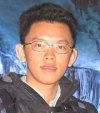
\includegraphics[height = 0.25\textheight]{halim.jpg}
% 		\begin{itemize}
% 			\item{Profesor de la Universidad Nacional de Singapur (UNS)}
% 			\item{Doctor en computación de la UNS}
% 			\item{Co-autor de los libros Competitive Programming 1 y 2}
% 			\item{Profesor del curso Competitive Programming en la NUS}
% 			\item{Entrenador del equipo de programación (ACM-ICPC) de la NUS y del equipo de la IOI de Singapur}
% 		\end{itemize}
% 	\end{frame}
% 	
% 	\begin{frame}
% 		\frametitle{Competitive Programming @ NUS}
% 		% \includegraphics[height = 0.25\textheight]{book.jpeg}
% 		\begin{itemize}
% 			\item{Curso creado en 2008 que busca fortalecer las habilidades de programación de sus estudiantes destacados para prepararlos para las competencias universitarias de programación de la ICPC}
% 			\item{Enfocado a estudiantes de tercer año con buenas habilidades de programación}
% 			\item{Curso avanzado, cubre muchos temas en poco tiempo}
% 			\item{Material abierto al público en \url{https://sites.google.com/site/stevenhalim/home/material}}
% 			\item \Large{\sout{Exámenes} $\rightarrow$ Competencias}
% 		\end{itemize}	
% 	\end{frame}
% 
% \section{Semillero de programación}
% 	\begin{frame}
% 		\frametitle{Semillero de programación - Eafit}
% 		\begin{itemize}
% 			\item Estudiantes interesados en mejorar sus habilidades de programación y competir en las maratones
% 			\item Estudiantes en su mayoría de 1ro y 3er semestre
% 			\item No tienen conocimiento previo de C++
% 			\item Reuniones semanales de 2 horas
% 		\end{itemize}
% 		
% 		\begin{center}
% 			\begin{tikzpicture}
% 				\draw [line width=3, ->] (0,0) -- (0,-1.1);
% 			\end{tikzpicture}\\
% 			\large{El semillero va más lento que el curso de la NUS} 
% 		\end{center}
% 	\end{frame}
% 	
% 	\begin{frame}
% 		\frametitle{Temas vistos}
% 		\begin{enumerate}
% 			\item{Introducción a los jueces de programación}
% 			\item{Introducción a C++ y a métodos de entrada y salida de datos}
% 			\item{Arreglos y Vectores en C++}
% 			\item{Representación de grafos: dirigidos, no dirigidos y con pesos}
% 			\item{Estructuras de datos: pila, cola, mapa, set y heap}
% 			\item{Recorrido de grafos: DFS y BFS}
% 			\item{Ordenamiento Topológico y Componentes Fuertemente Conexas}
% 			\item{Algoritmo de Dijkstra}
% 		\end{enumerate}
% 	\end{frame}
% 	
% 	\begin{frame}
% 		\frametitle{Problemas propuestos}
% 		\begin{itemize}	
% 			\item Luego de explicar cada tema se dejan como tarea un conjunto de problemas que apliquen los temas aprendidos.\\
% 			\item Los problemas de las competencias se escogen de los problemas propuestos en el libro de Steven Halim.\\
% 			\item Se resuelven los problemas antes de proponérselos como ejercicio a los estudiantes.
% 		
% 		\end{itemize}
% 	\end{frame}
% 	
% 	\begin{frame}{Competencias}
% 		\begin{itemize}
% 			\item Al igual que en el curso de la NUS, se hacen competencias competencias con los problemas propuestos.
% 			\item Las competencias se hacen utilizando el sitio \url{http://contests.factorcomun.org/}\\
% 			\item Estas comienzan al acabar la reunión y terminan al inicio de la siguiente, donde se discuten y resuelven los problemas.\\
% 			\item Con las competencias se mide el nivel de los estudiantes, esto permite ajustar el nivel de los temas.
% 		\end{itemize}
% 	\end{frame}
% 	
% 	
% 	\begin{frame}
% 		\frametitle{Competencias}
% 		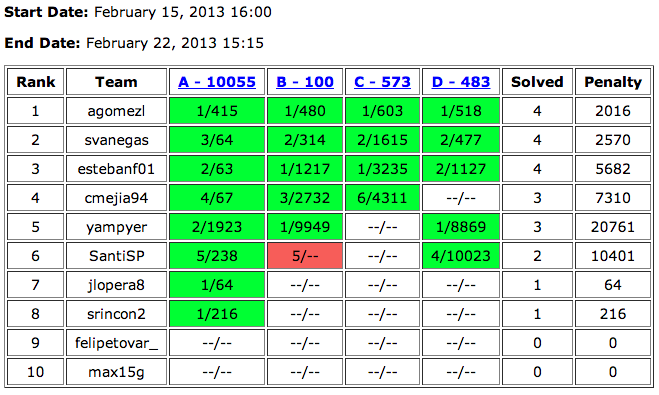
\includegraphics[width = 0.95\textwidth]{contest.png}
% 	\end{frame}
% 	
% 	\begin{frame}
% 		\frametitle{Competencias}
% 		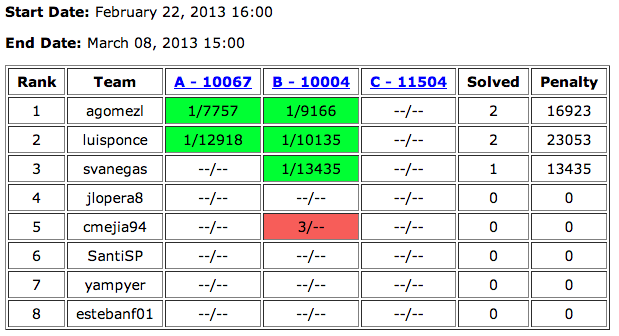
\includegraphics[width = 0.95\textwidth]{contest2.png}
% 	\end{frame}
% 
% % \section{Bibliografía}
% % 	\begin{frame}[allowframebreaks]
% % 		\frametitle{Bibliografía}
% % 		\bibliographystyle{plain}
% % 		\bibliography{Biblio}
% % 	\end{frame}
% 	
\section{Preguntas}
	\begin{frame}
		\frametitle{Preguntas}
		
\includegraphics[width = 0.9\textwidth]{preguntas.jpeg}
	\end{frame}

\end{document}